\documentclass[conference]{IEEEtran}
\usepackage[utf8]{inputenc}
\usepackage[T1]{fontenc}
\usepackage{graphicx} % Required for including images
\usepackage{amsmath} % Required for math commands
\usepackage{booktabs} % Required for professional looking tables
\usepackage{float} % Required for tables and figures positioning
\usepackage{xcolor} % Required for color definitions
\usepackage{afterpage}

\definecolor{myblue}{HTML}{717AFD}
\definecolor{myred}{HTML}{F0564A}
\definecolor{mygrey}{HTML}{464546}

\setlength{\parskip}{0.8em} % Adjust space between paragraphs

% Formula example $V=5\,\rm{V}$

\newcommand\wordcount{
   \immediate\write18{wordcount.bat \jobname.tex}
   \input{\jobname.wc}
}

\begin{document}

\title{Guided sensors report}
\author{Blind grading number 2504F}
\maketitle

\section{General Introduction} % 500 words
% Open source hardware save the world\cite{BiomakerOrg2022}. and cite also Arduino
Technology has become an essential part of our daily lives. 
At work, for leisures or health check-ups, we interact with complex devices that, 
thanks to their user-friendly interfaces, do not require us to understand the 
undearneath mechanisms. This often leads us to perceive tools as telephones or 
computers as `black boxes' that magically performs tasks - while they are 
assemblies of simple technologies finely tuned together.

Making hardware open-source is essential to demistify such a perception. In the 
field of electronics, the open-source philosophy (defined by a design that is made 
publicly available, allowing anyone to study, modify, distribute, make, and sell 
it \cite{dosemagenGatheringOpenScience2017} - in striking contrapposition to the 
`patent' way of operating) has been boosted and gained further recognizion with 
widely spread projects such Arduino \cite{ArduinoHome} or Raspberry Pi 
\cite{foundationTeachLearnMake2023}. Not only those projects have made the 
learning curve less steep, but also cheapened the prototype phase of device building.

A natural extension of open-source hardware is the Do-It-Yourself (DIY) movement: 
thanks to the shared knowledges and designs, individuals are empowered to build, 
customize and repair electronic devices independently. Bulky and expensive machines 
such as thermocyclers can be then `hacked' and readapted to fit in a pocket 
\cite{PocketPCRGaudiShop}, or engineered to be constructed by over-the-self 
electronics and 3D printing \cite{AirFlowMicroreactor}; 

Sensors are a class of electronic devices which became daily use in the 
last years. While sensors as pulse and glucose meters, or self-test for 
diagnosis (as the ones for Covid-19) are already of common use, in the next years 
we will benefit from "wereable" non-invasive sensors for continous monitoring of 
health parameters \cite{smithReshapingHealthcareWearable2023}, or quick detection of 
allergenes in our food \cite{sundhoroRapidAccurateElectrochemical2021}. Keeping 
those technologies open-source will assure that they stay \textit{for} individuals and \textit{by}
individuals.

Here, we provide two examples of open-source DIY sensors. First, we improve 
the accurancy of a commercial temperature sensor by customazing the current design 
with analog amplification circuits; a calibration protocol is also be provided. 
This is a proof of concept of how open-source technology allows for continuous 
improvement and refining by the community. Secondly, we construct from scratch 
a pulse meter starting simply from the understanding of the mechanisms 
needed, providing an example of completely DIY technology.


% Open source hardware and DIY
% Sensors are not a black box
\section{Temperature Sensor} % 1000 words
   \subsection{Introduction and goals}
   \subsection{Sensor design}
      \subsubsection{Electronic diagram}
         The complete circuit diagram is shown in Figure \ref{fig:circuit}. Overall, the designed circuit was divided into 4 parts:

         \begin{enumerate}
            \item A DAC module that converts the PWM current from the Arduino into a continuous voltage, which is fed into the positive 
               pin of the Operational Amplifier, simulating the voltages that the sensor will generate later. After experimental testing of
               the circuit and measuring it with an oscilloscope (results not shown), it was established that the resistance of the low-pass
               filter of the DAC should be as low as possible (100 Ohms finally) so that the relationship between its resistance and the
               rest of the rail (especially resistors $R_4 + {R_3} / {R_2}$) is low enough to obtain most of Vin at the output of the
               DAC (otherwise, a significant potential would drop across the DAC resistor). This circuit is connected or disconnected
               through the mosfet D5.

            \item The amplification circuit is composed of an operational amplifier working as a voltage amplifier, and two interchangeable
               circuits to select gains of 2.2X or 22X. These circuits are activated with digital pins D2 and D3, and they change the resistances
               in the loop and in the positive rail. The latter facilitates the use of offset removal, which is subtracted in a 1:1 ratio
               (the applied offset is the same as subtracted from the sensor's value).

            \item The offset removal, controlled through the Arduino's internal DAC on pin A0 with a precision of 12 bits and a range of 0-4.7V
               (when the Arduino is connected via USB), providing a theoretical step of 1mV. The offset is applied to the inverting input and undergoes
               the same type of resistance as the sensor voltage to apply a 1:1 subtraction.

            \item The noise filtering circuits, consisting of a 100nF decoupling capacitor and a low-pass filter at the output of the Operational
               Amplifier, which are responsible for filtering high frequencies from the microcontroller crystals, both in the voltage rail and at
               the output of the operational amplifier.

            \item The sensor connector, where the MCP9001 is plugged into the system.
         \end{enumerate}

         \begin{figure*}[!th]
            % \afterpage{\clearpage}
            \centering
            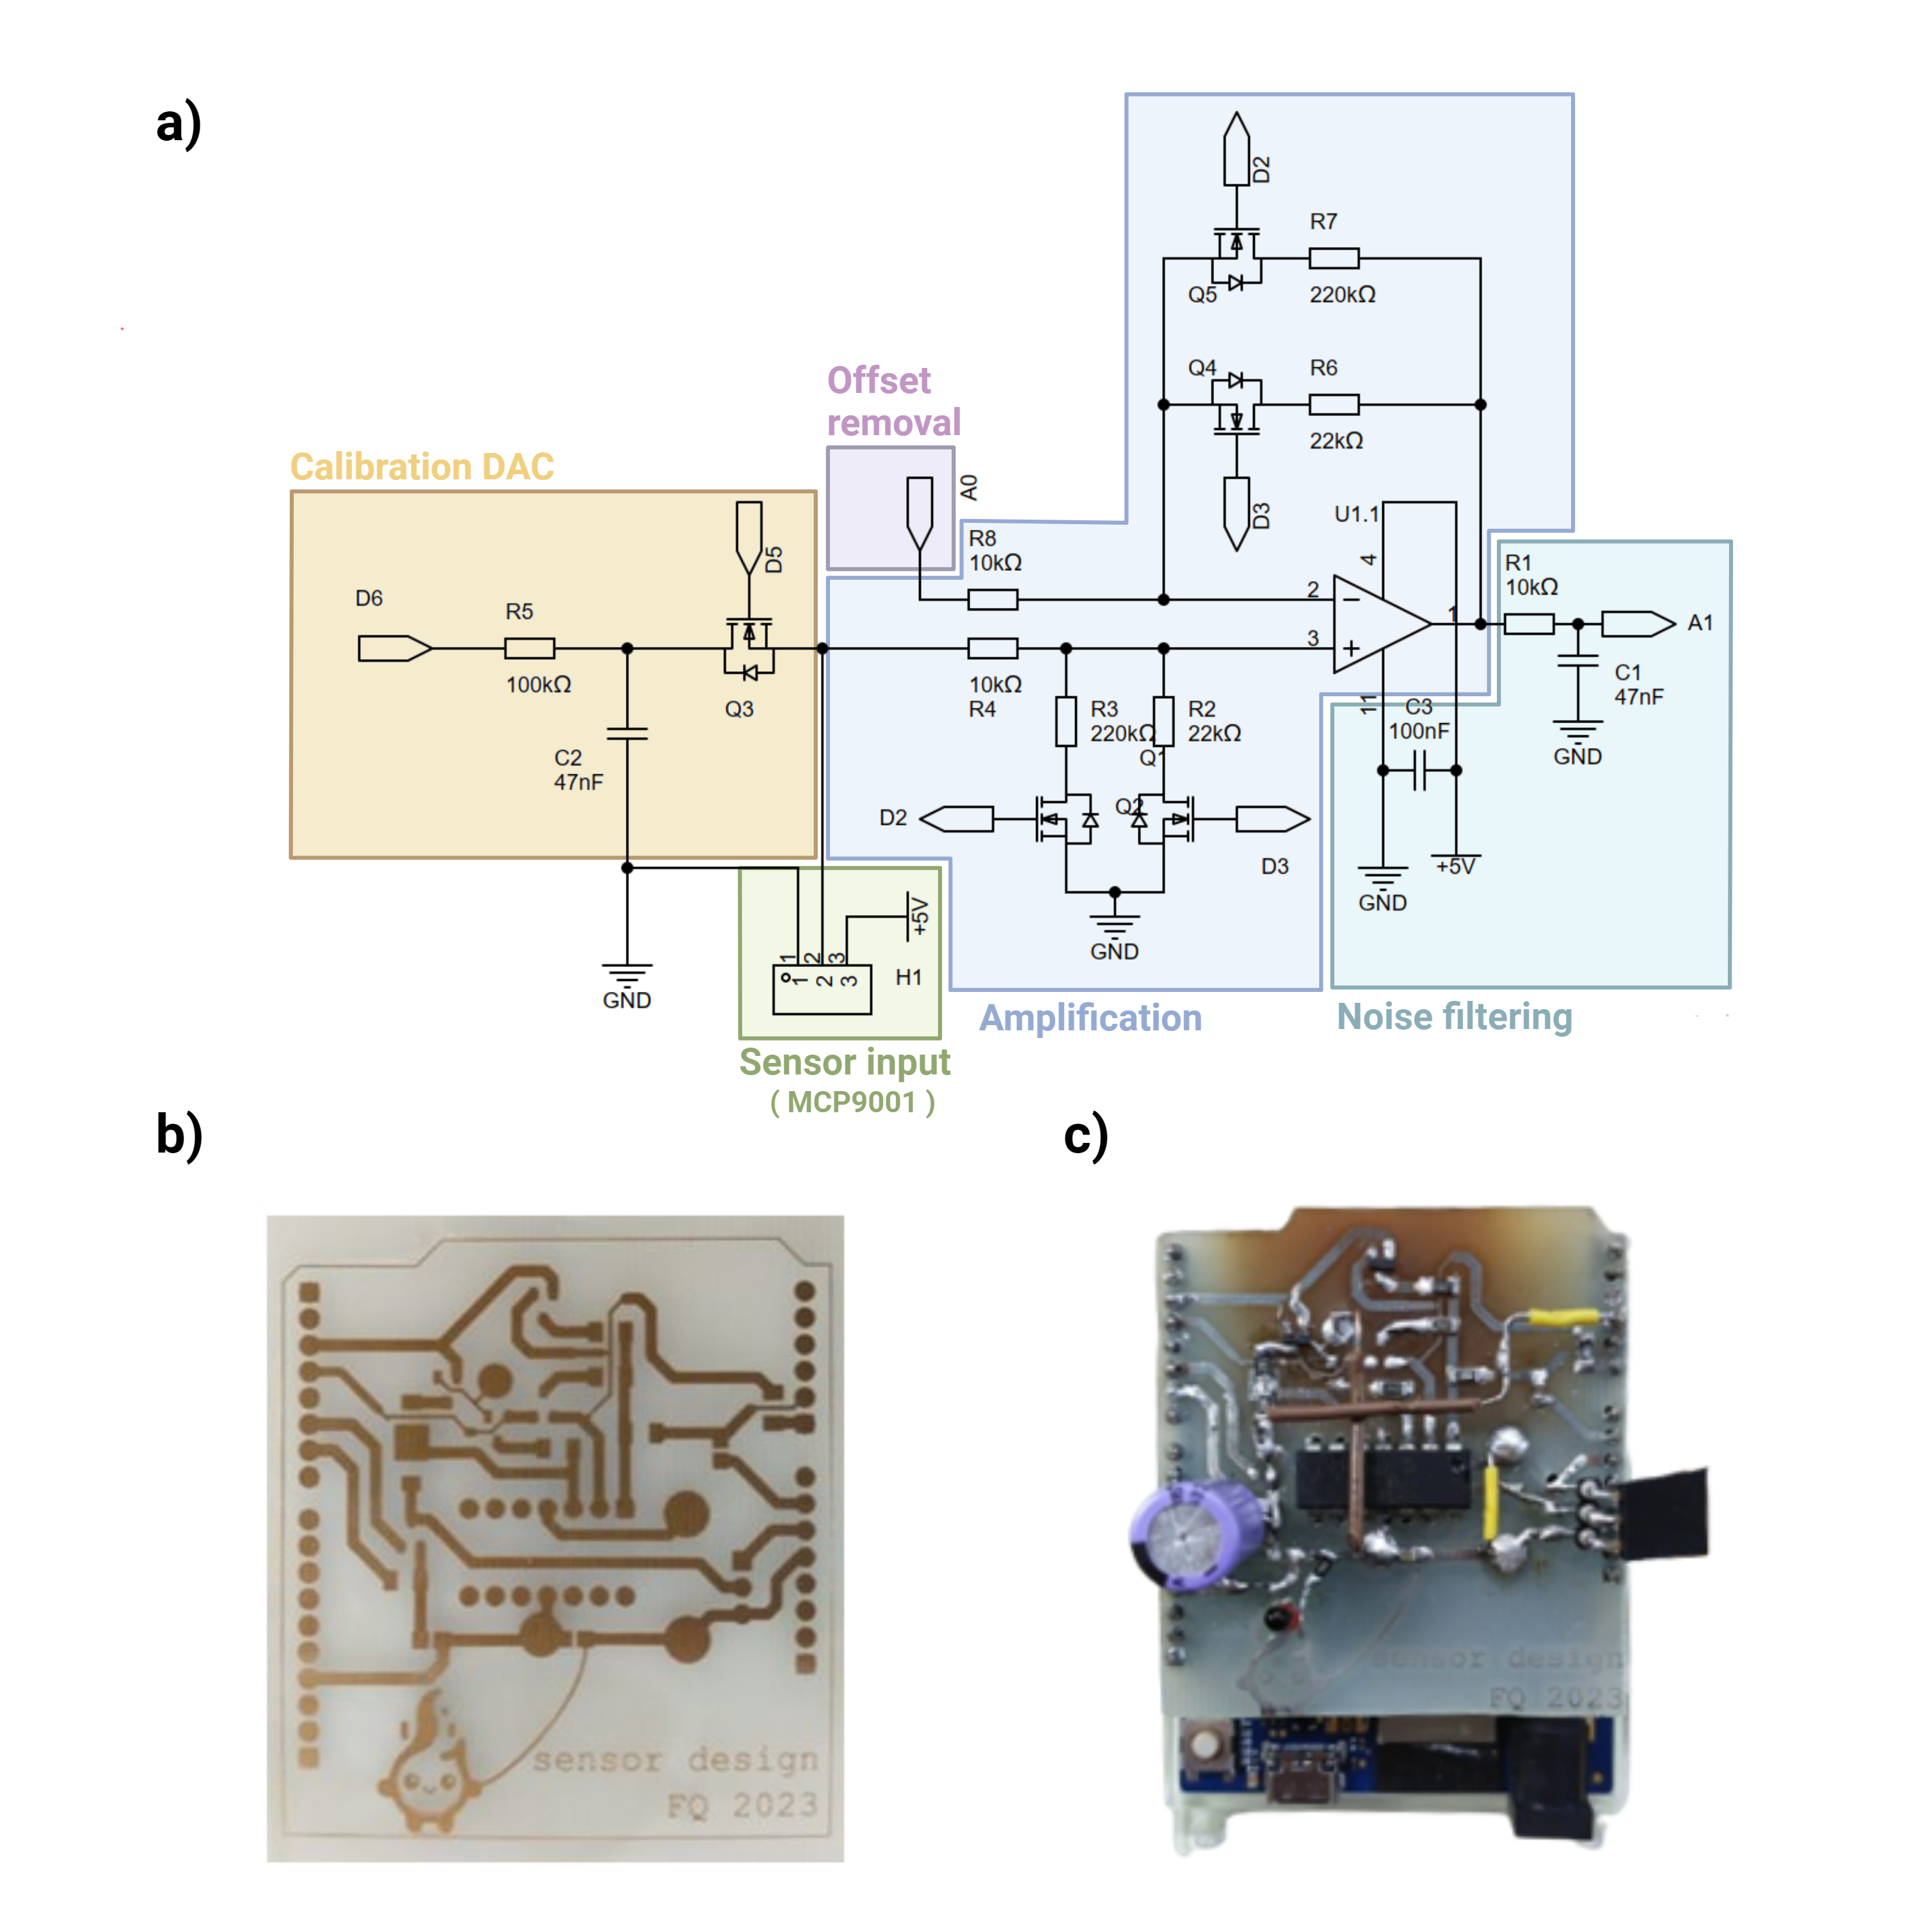
\includegraphics[width=\textwidth]{images/electronic_diagram.png}
            \caption{Annotated electronic diagram (a), etched PCB (b) and PCB after soldering and rework (c).}
            \label{fig:circuit}
         \end{figure*}

         % \clearpage

      \subsubsection{Electronics production}
      The circuit schematics were created in EasyEDA. The Arduino UNO Shield templates were imported from OpenSourceHardware Lab \cite{ArduinoShieldEasyEDA}.
      Printed circuit boards (PCBs) with pre-routed traces were printed on transparent projection films and aligned on a single-side copper board covered by a positive photomask.
      The PCBs were exposed to UV light for 5 minutes, followed by a sodium hydroxide bath to remove excess mask. Subsequently, the copper plates were immersed in a copper etchant solution (Ferric Chloride)
      to remove the copper from the exposed regions. Finally, the mask was removed with acetone, and the plates were immersed in thiourea to coat the copper with a layer of tin.
      \subsubsection{Sensor probe}
      The sensor was soldered to solid core wires and made waterproof using a combination of heat-shrink plastic and heat-shrink tubing. Two layers were added
      to ensure insulation, guaranteeing that the ceramic surface remained exposed to facilitate thermal exchange.
      \subsection{Sensor Calibration}
      To attempt to isolate the origin of any potential error, the operational amplifier was first calibrated (and its error studied), and then the output of the 
      operational amplifier was mapped against a digital reference temperature sensor (HH802WE, Omega).

      \subsubsection{Operational Amplifier Calibration}
      Initially, a sweep was performed with the calibration DAC from 0 to a saturation voltage (4.7V), first activating the gain 2 loop circuit and then the gain 22 circuit.
       After confirming that both circuits worked by comparing the obtained gains (and the amplification range) with the expected values, a "sequential offset subtraction" code 
       (using the Arduino's internal DAC) was implemented to subtract a discrete offset each time the operational amplifier was saturated (Appendix A; Figure \ref{fig:opamp}a). The results gradually show that as the 
       removed offset increases, a minimum in the output voltage is reached, beyond which the signal cannot decrease(Appendix A; Figure \ref{fig:opamp}b). The potential explanation for this voltage lies in the internal
        diode of the operational amplifier closed-loop MOSFETs. Even when the MOSFET is open, not conducting voltage through the loop from the output of the operational amplifier 
        to the inverting input, the internal diode of the MOSFET allows circulation from the inverted input of the op-amp to the op-amp's output, contaminating this output with the DAC voltage. 
        When the offset voltage is small, most of it falls on the diode, but as the output grows, it becomes more and more contaminated. Some specialized forums suggest using "back-to-back" MOSFETs\cite{BackBackMOSFET} 
        as a potential solution, but after a quick attempt, the result remained the same. Therefore, due to time constraints, it was decided to desolder the 2X loop and continue the experiment only with a 
        gain of 22, whose results, along with the offset subtraction script, showed an effective input range from 0 to 4.7 volts with an output (including the subtracted offset from the sensor voltage) 
        of approximately 0-104V(Figure \ref{fig:finalop}).

        \begin{figure}[h]
         \centering
         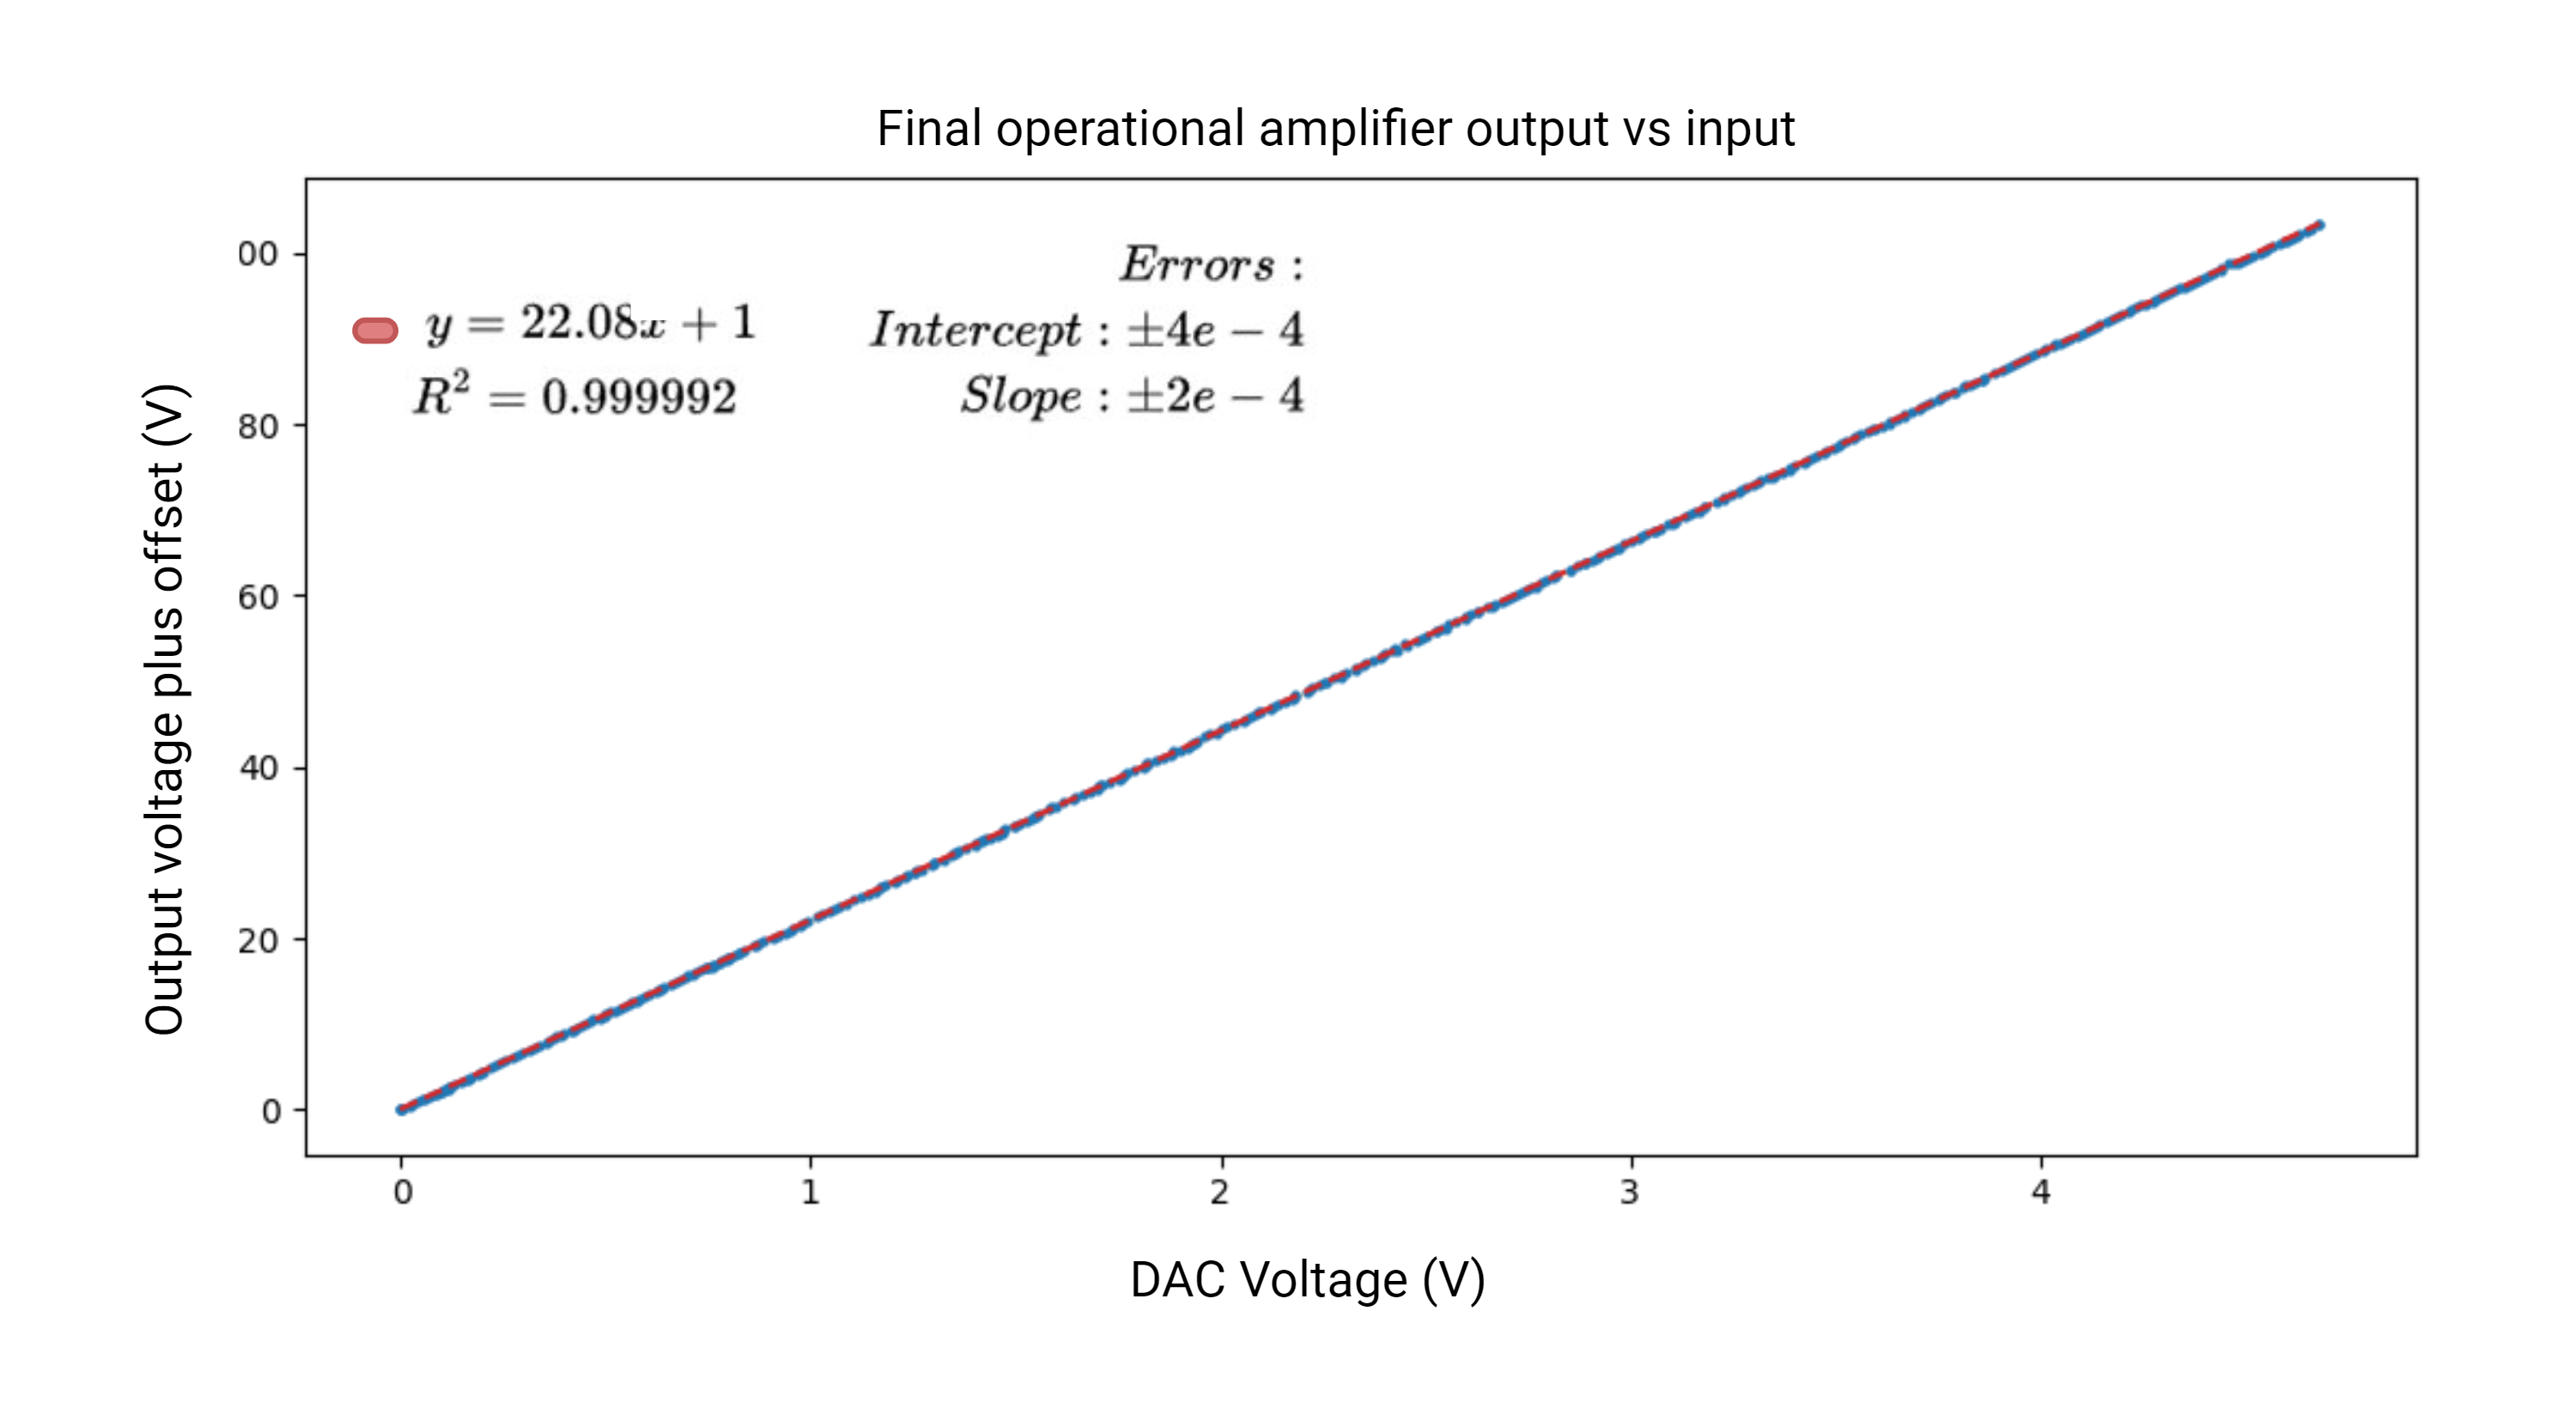
\includegraphics[width=1\linewidth]{images/finalop.png}
         \caption{Final plot of DAC voltage vs. the output operational amplifier voltage after adding the offset.}
         \label{fig:finalop}
      \end{figure}

      \subsubsection{Temperature calibration}

      For temperature calibration, a previously published open-source isothermal fluorimeter was modified \cite{Open_qLAMPMasterOpen2023}.
      The heated lid was separated from the housing and folded around the two sensors, creating the equivalent of a 'spring roll' with the two sensors 
      in the center and the lid spiraling around them (Figure \ref{fig:temp}a). The lid was then heated at different intensities, after which it was allowed to reach thermal 
      equilibrium for 3-4 minutes, and the voltage value at the output of the operational amplifier and the temperature of the reference sensor were recorded. 
      A linear regression was then established, and the error was studied reaching a value of ~±1°C (Figure \ref{fig:temp}b).
      
      \begin{figure}[h]
         \centering
         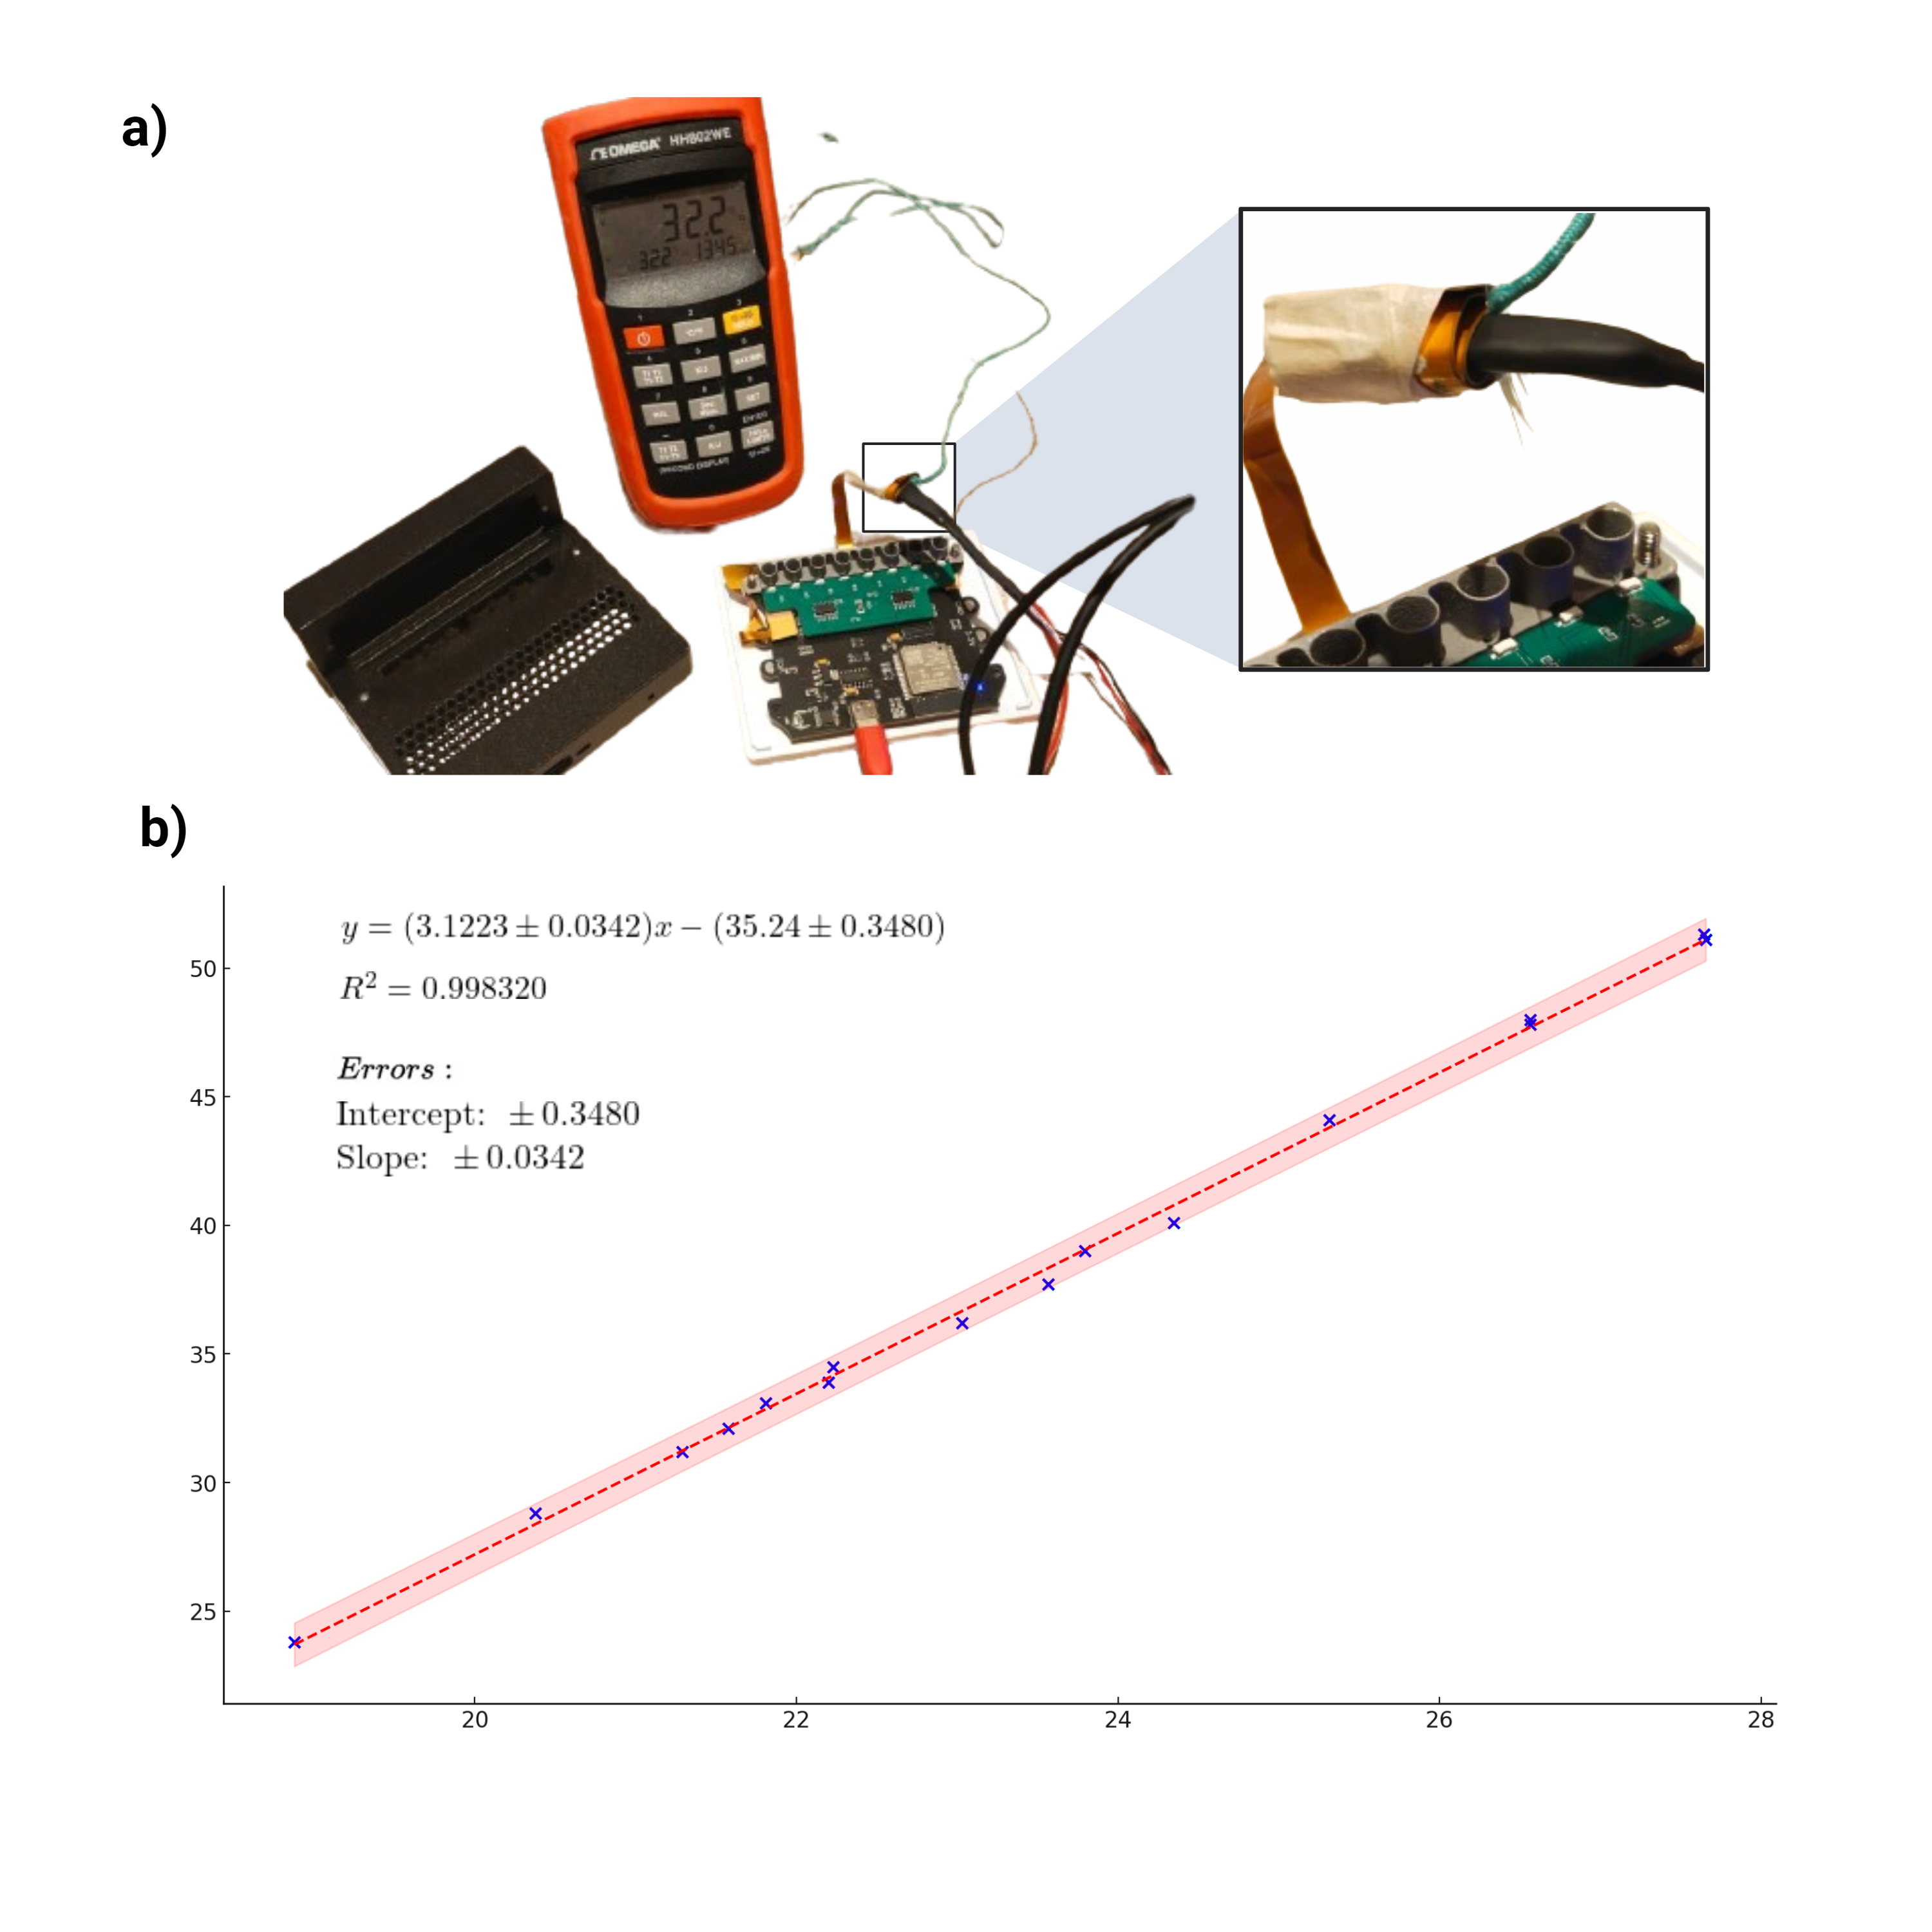
\includegraphics[width=1\linewidth]{images/temp calibration.png}
         \caption{Temperature calibration setup (a) and results (b)}
         \label{fig:temp}
      \end{figure}


   \subsection{Results and discussion}

   Finally, the sensor was tested against the reference method to measure a dynamic system, the cooling of freshly boiled water from 95°C to 25°C. Both sensors were coiled together and secured with thermally conductive tape. 
   They were submerged in the water, and the temperature was continuously recorded and plotted with a linear correlation analysis (Figure \ref{fig:final}).

\begin{figure}[h]
    \centering
    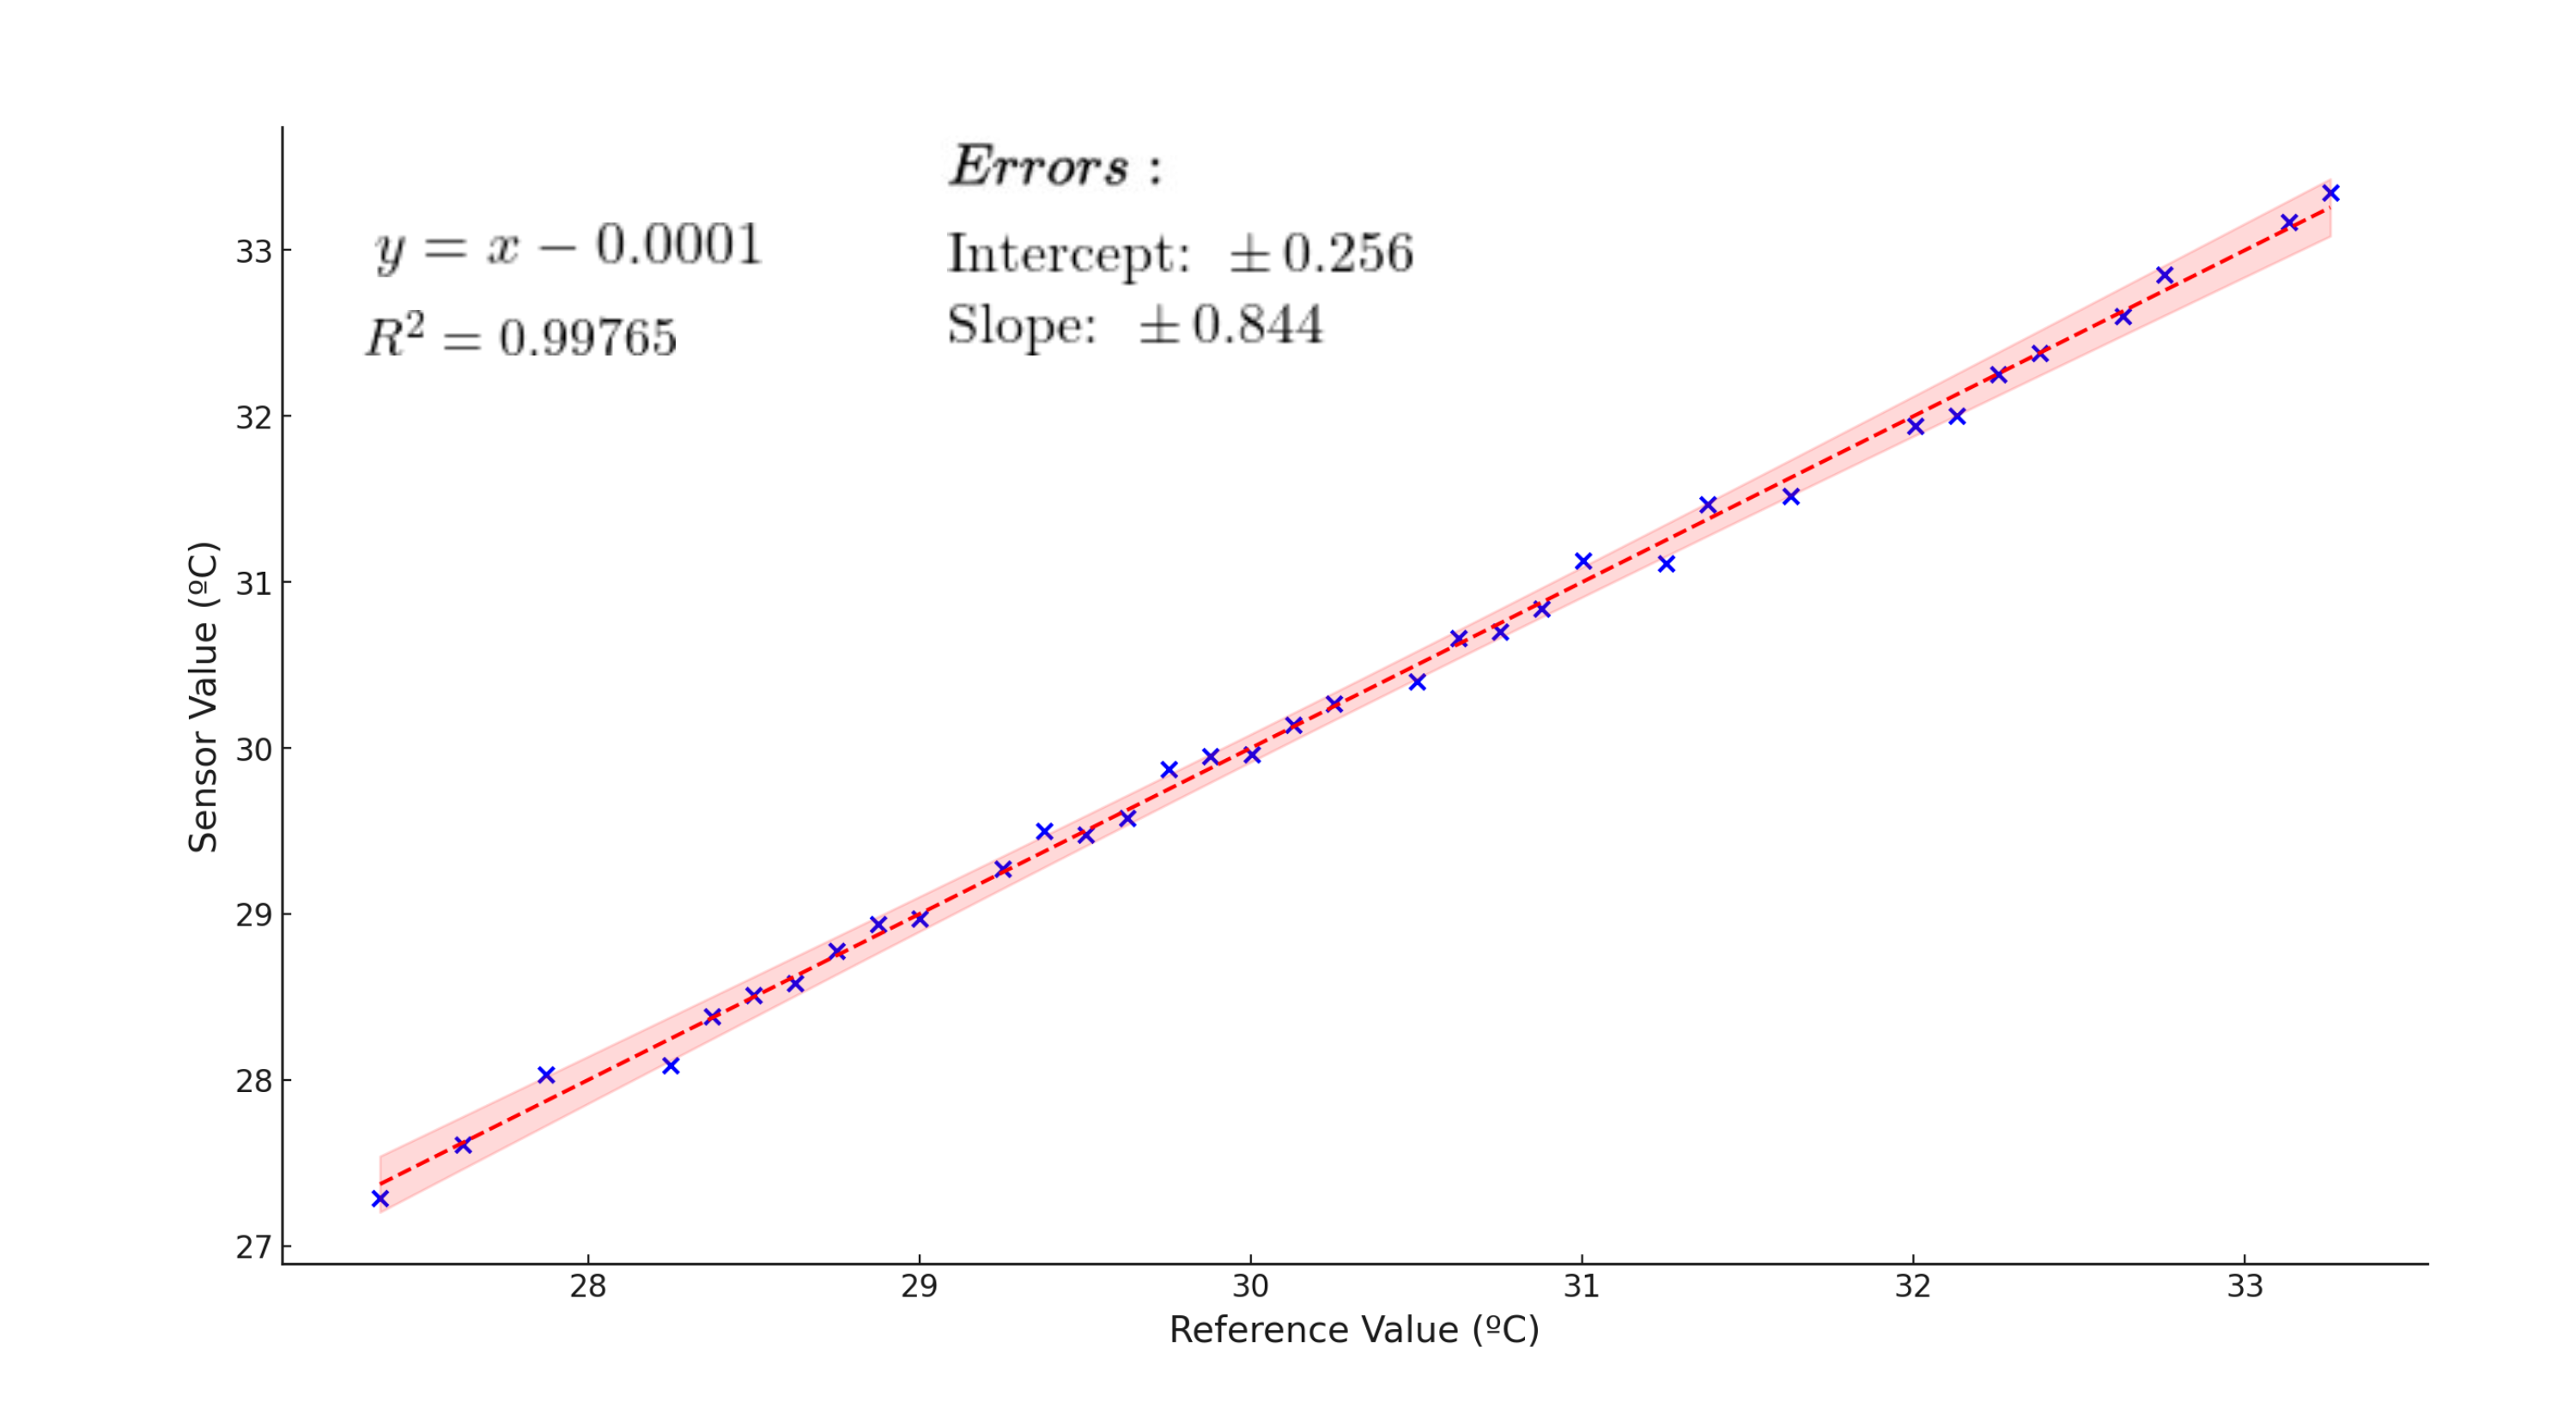
\includegraphics[width=1\linewidth]{images/final results.png}
    \caption{}
    \label{fig:final}
\end{figure}

In these results, the following observations can be made:
\begin{enumerate}
    \item Both methods have a correlation with a slope of 1 and an intercept almost equal to 0, indicating high accuracy.
    \item Considering the error, the maximum difference between values is approximately ±1°C (Accuracy of ~±1°C).
    \item Taking into account that the error of the operational amplifier during the calibration step was nearly negligible, and the final error is nearly the same as the one obtained in the sensor calibration against a reference method, we can conclude that the bottleneck for improving accuracy is the replicability of the temperature sensor's results itself.
    \item The results of the adaptive offset circuit are satisfactory, potentially allowing for higher amplification without limiting the range. However, considering the accuracy results of the sensor (the variability obtained around the same temperature), it does not seem that increased amplification would solve the problem.
\end{enumerate}

\section{Pulse meter} % 1000 words
   \subsection{Introduction and goals}
   \subsection{Sensor design}
      \subsubsection{Electronic diagram}
      \subsubsection{Sensing probes}
      \subsubsection{Case}
      \subsubsection{User Interface}
      \subsubsection{Results and conclusion}
\section{General Conclusion} % 500 words




\bibliographystyle{IEEEtran}
\bibliography{guided_sensor}

% Uncomment the compliance section if you have set it up properly
\section{Compliance}
\wordcount
\appendices
\begin{figure*}[h]
   \centering
   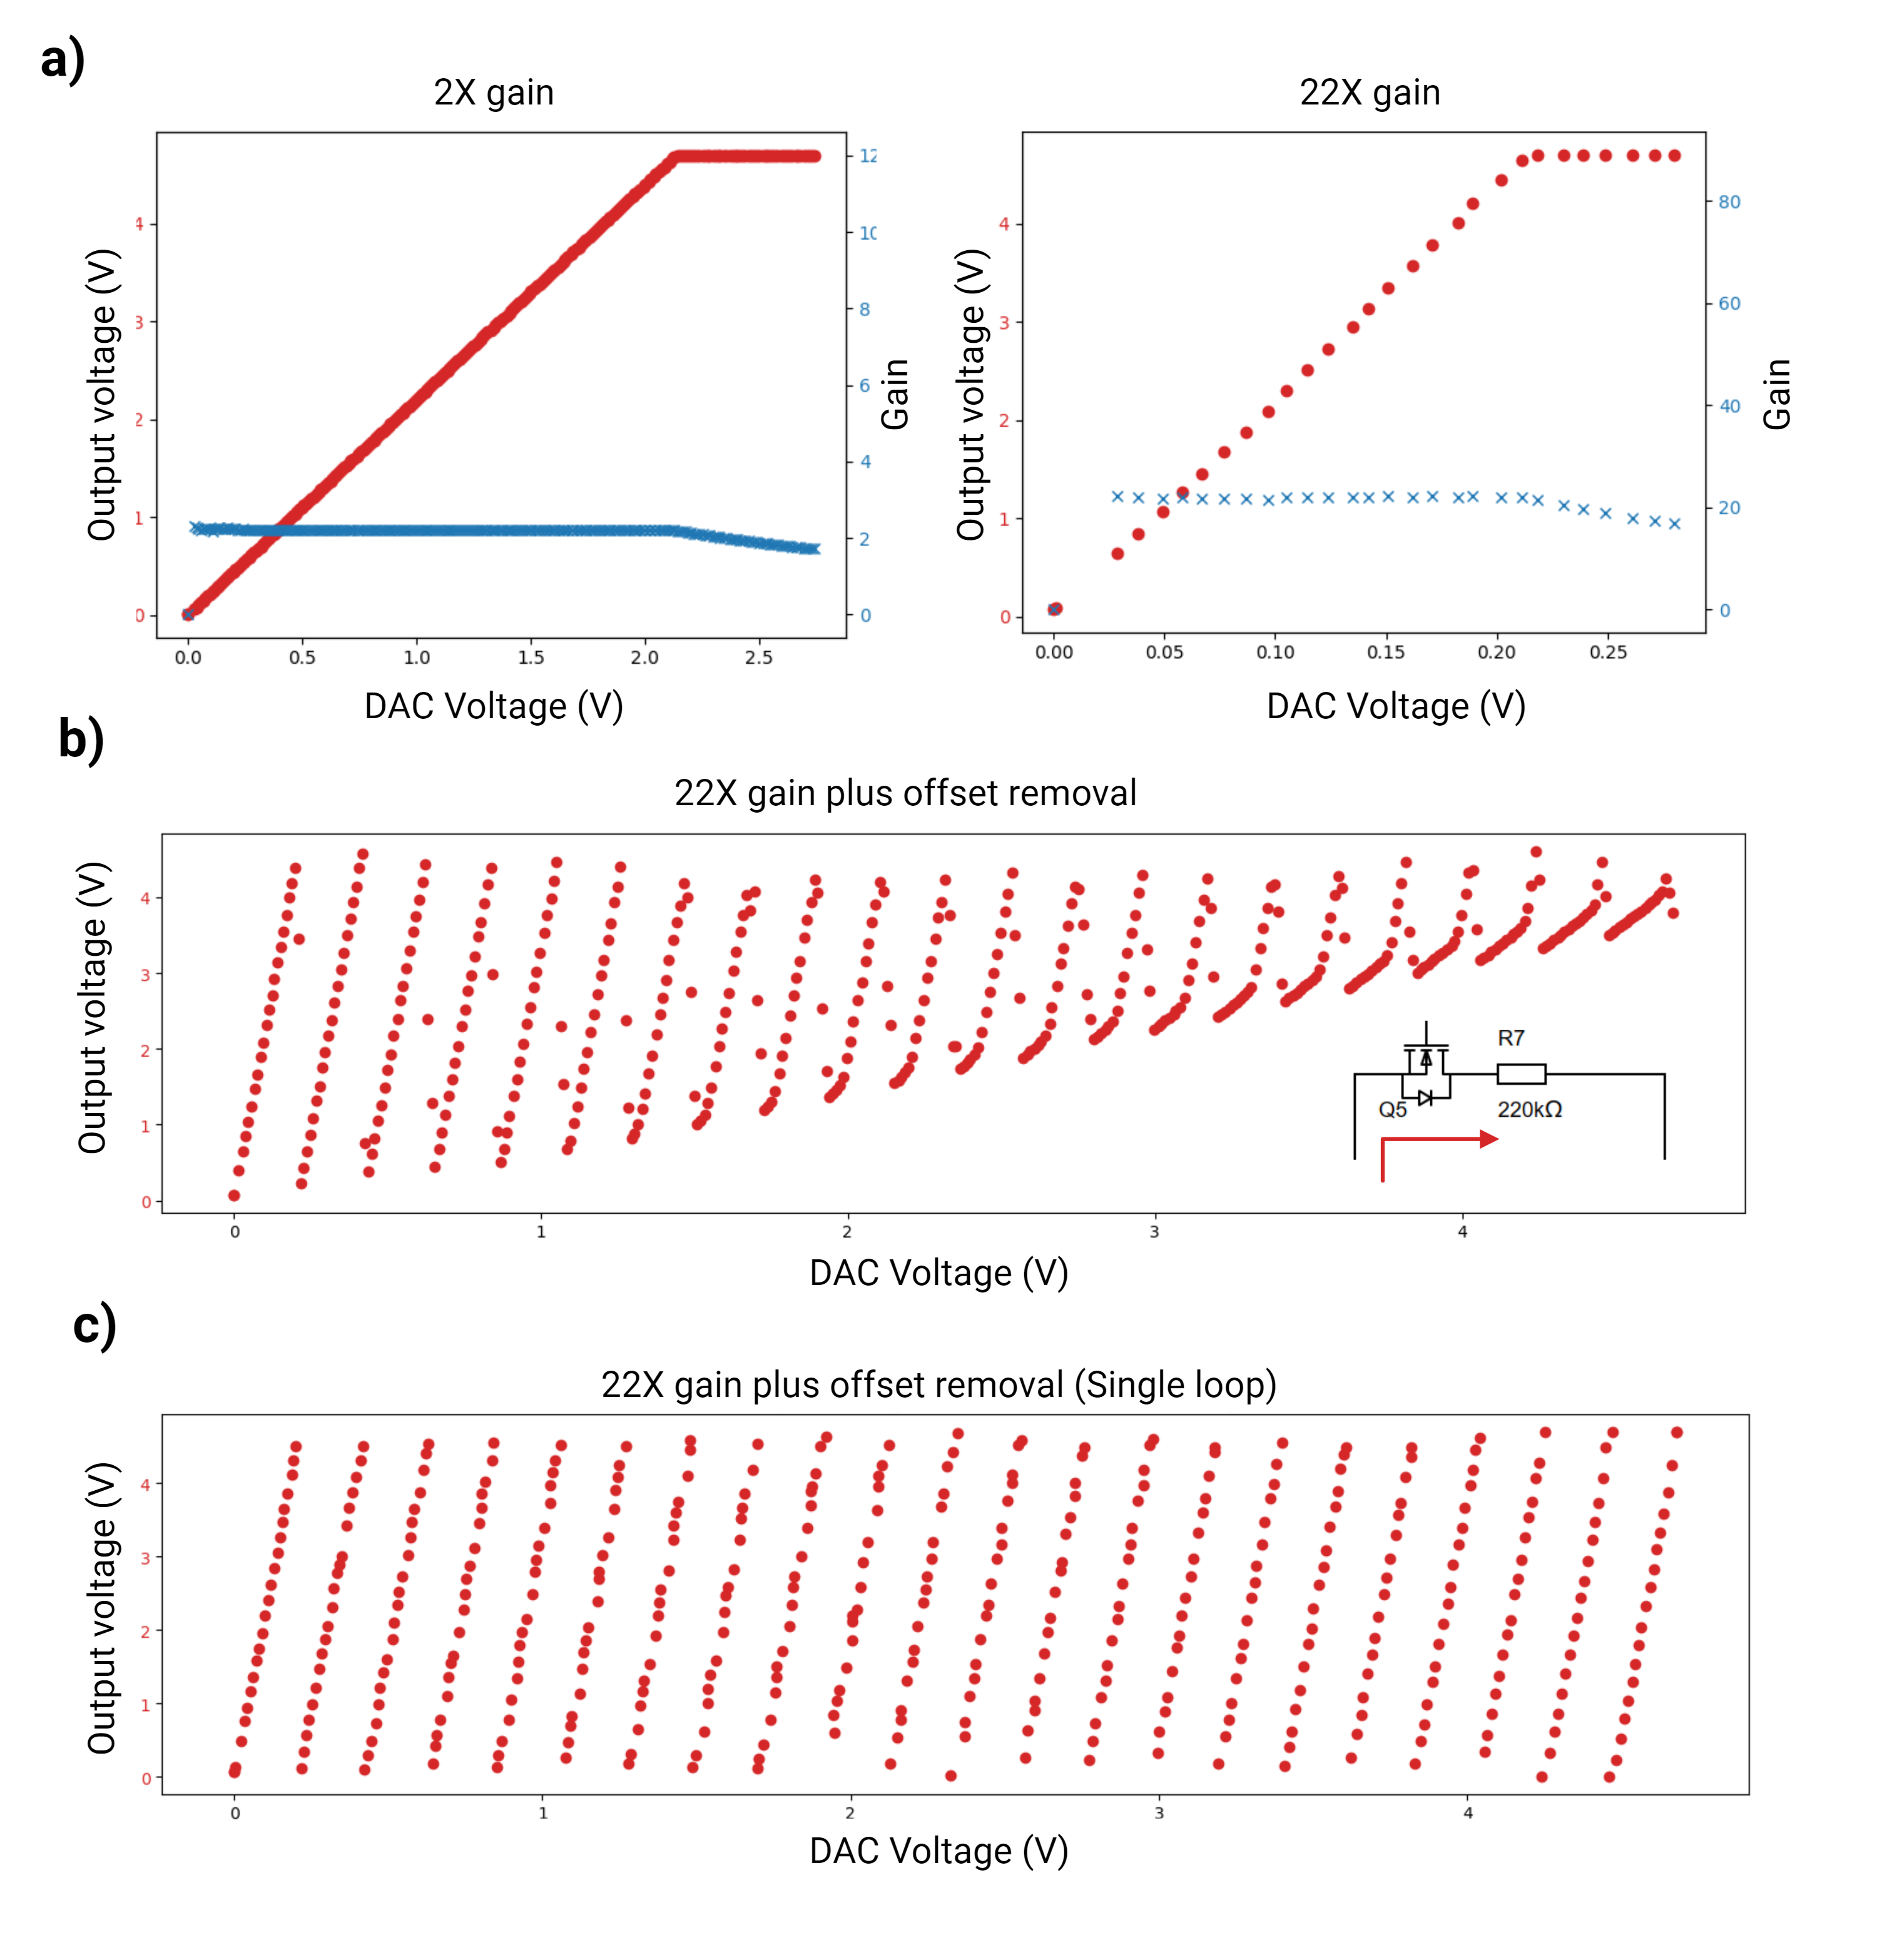
\includegraphics[width=\textwidth]{images/op amp calibration.png}
   \caption{Operational amplifier calibration. Demonstration of the closed-loop resistance exchange circuit without offset removal (a).
   Introduction of offset removal and the appearance of a minimum reachable voltage (b), which is resolved upon removing the MOSFET from the gain 2 closed-loop (c).}
   \label{fig:opamp}
\end{figure*}

\end{document}
